\pdfminorversion=4
\documentclass[aspectratio=169]{beamer}

\mode<presentation>
{
  \usetheme{default}
  \usecolortheme{default}
  \usefonttheme{default}
  \setbeamertemplate{navigation symbols}{}
  \setbeamertemplate{caption}[numbered]
  \setbeamertemplate{footline}[frame number]  % or "page number"
  \setbeamercolor{frametitle}{fg=white}
  \setbeamercolor{footline}{fg=black}
} 

\usepackage[english]{babel}
\usepackage[utf8x]{inputenc}
\usepackage{tikz}
\usepackage{courier}
\usepackage{array}
\usepackage{bold-extra}
\usepackage{minted}
\usepackage[thicklines]{cancel}
\usepackage{fancyvrb}

\xdefinecolor{dianablue}{rgb}{0.18,0.24,0.31}
\xdefinecolor{darkblue}{rgb}{0.1,0.1,0.7}
\xdefinecolor{darkgreen}{rgb}{0,0.5,0}
\xdefinecolor{darkgrey}{rgb}{0.35,0.35,0.35}
\xdefinecolor{darkorange}{rgb}{0.8,0.5,0}
\xdefinecolor{darkred}{rgb}{0.7,0,0}
\definecolor{darkgreen}{rgb}{0,0.6,0}
\definecolor{mauve}{rgb}{0.58,0,0.82}

\title[2021-05-04-hllhc-workshop]{Python Data Science}
\author{Jim Pivarski}
\institute{Princeton University -- IRIS-HEP}
\date{May the 4$^{\mbox{\scriptsize th}}$ be with you}

\usetikzlibrary{shapes.callouts}

\begin{document}

\logo{\pgfputat{\pgfxy(0.11, 7.4)}{\pgfbox[right,base]{\tikz{\filldraw[fill=dianablue, draw=none] (0 cm, 0 cm) rectangle (50 cm, 1 cm);}\mbox{\hspace{-8 cm}
\includegraphics[height=1 cm]{princeton-logo-long.png}\hspace{0.1 cm}\raisebox{0.1 cm}{
\includegraphics[height=0.8 cm]{iris-hep-logo-long.png}}\hspace{0.1 cm}}}}}

\begin{frame}
  \titlepage
\end{frame}

\logo{\pgfputat{\pgfxy(0.11, 7.4)}{\pgfbox[right,base]{\tikz{\filldraw[fill=dianablue, draw=none] (0 cm, 0 cm) rectangle (50 cm, 1 cm);}\mbox{\hspace{-8 cm}
\includegraphics[height=1 cm]{princeton-logo.png}\hspace{0.1 cm}\raisebox{0.1 cm}{
\includegraphics[height=0.8 cm]{iris-hep-logo.png}}\hspace{0.1 cm}}}}}

% Uncomment these lines for an automatically generated outline.
%\begin{frame}{Outline}
%  \tableofcontents
%\end{frame}

% START START START START START START START START START START START START START

\begin{frame}{}
\LARGE
\begin{center}
\textcolor{darkblue}{Part 1: Trends in data analysis software}
\end{center}
\end{frame}

\begin{frame}{Pythonic data analysis in the HL-LHC era?}
\vspace{0.25 cm}
\begin{center}
\only<1>{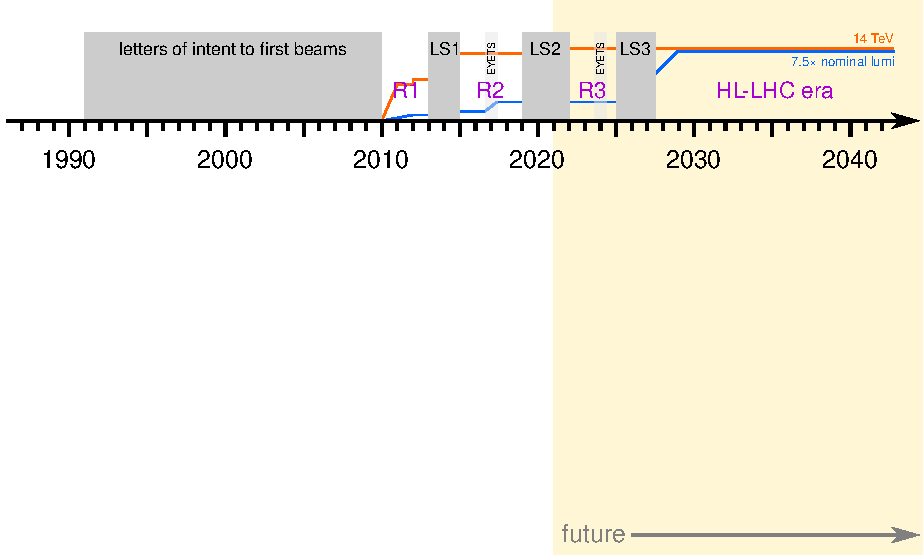
\includegraphics[width=0.9\linewidth]{hllhc-python-timeline-0.pdf}}\only<2>{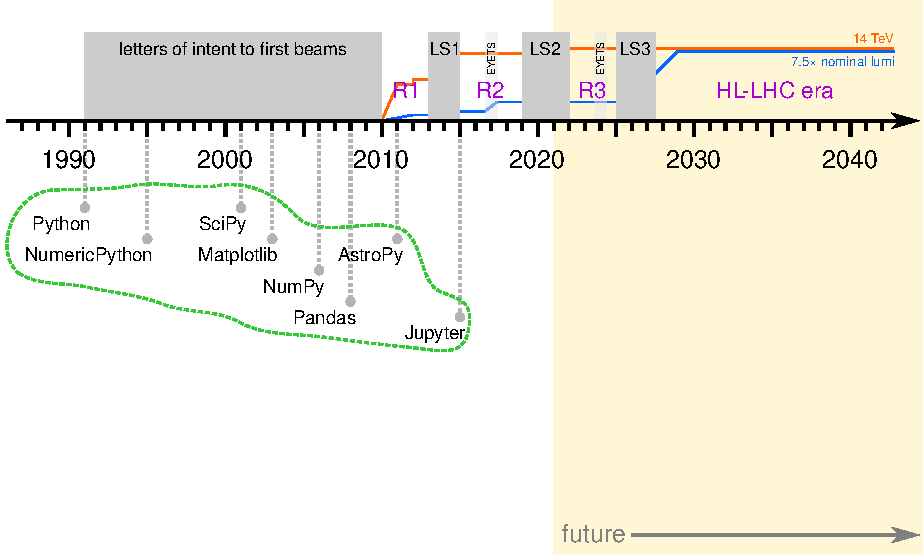
\includegraphics[width=0.9\linewidth]{hllhc-python-timeline-1.pdf}}\only<3>{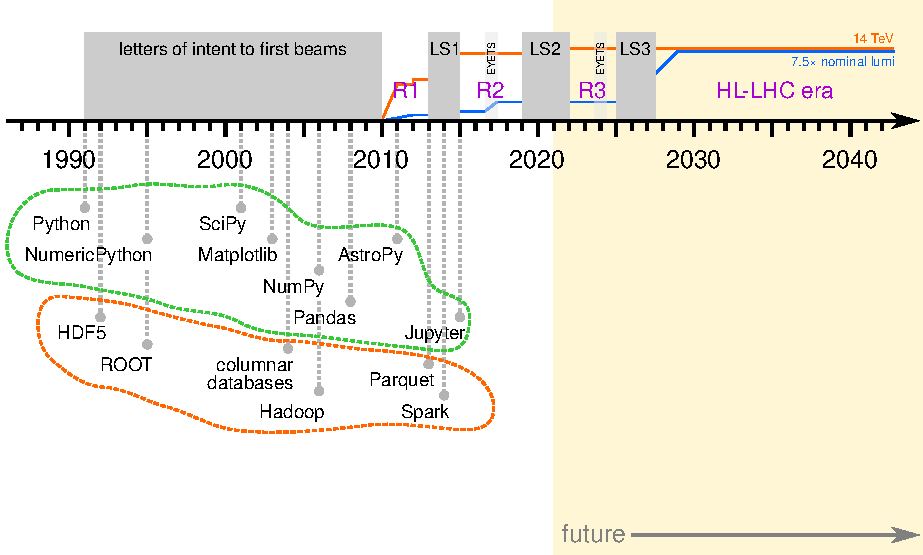
\includegraphics[width=0.9\linewidth]{hllhc-python-timeline-2.pdf}}\only<4>{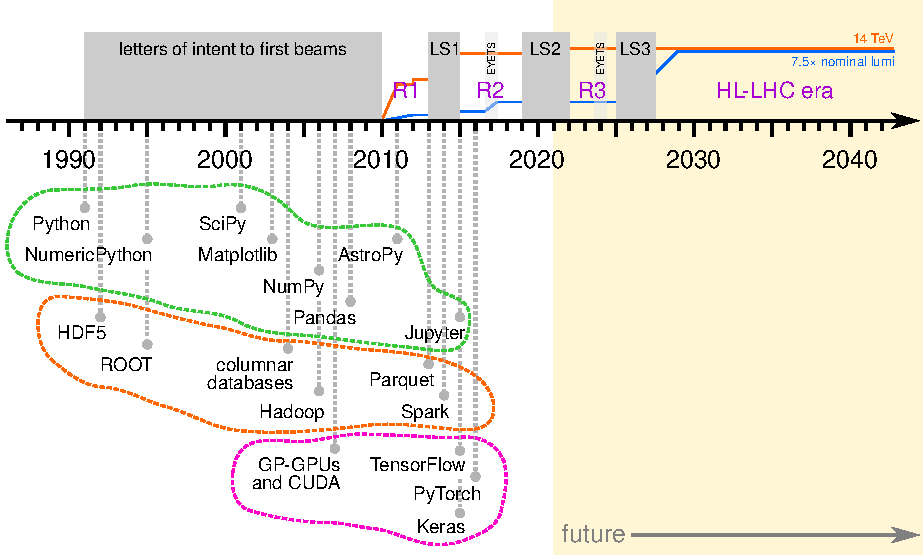
\includegraphics[width=0.9\linewidth]{hllhc-python-timeline-3.pdf}}\only<5>{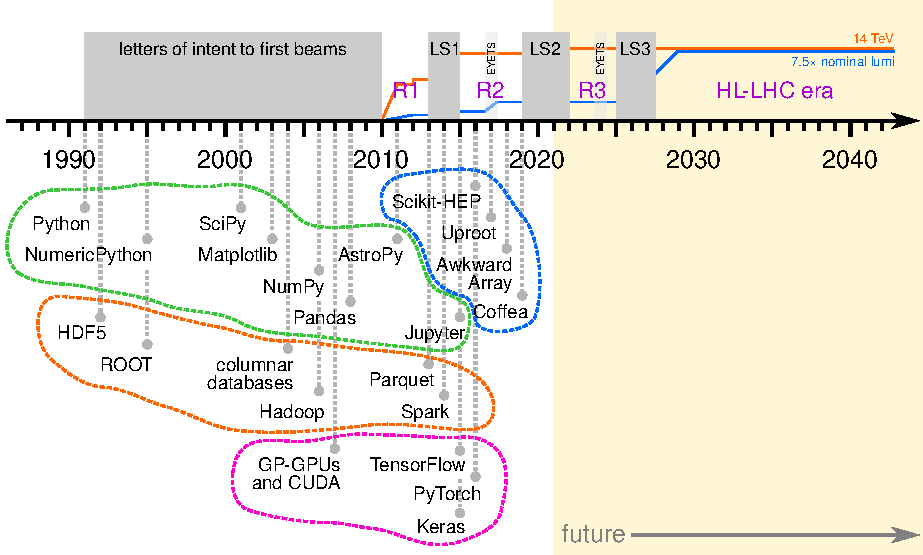
\includegraphics[width=0.9\linewidth]{hllhc-python-timeline-4.pdf}}\only<6>{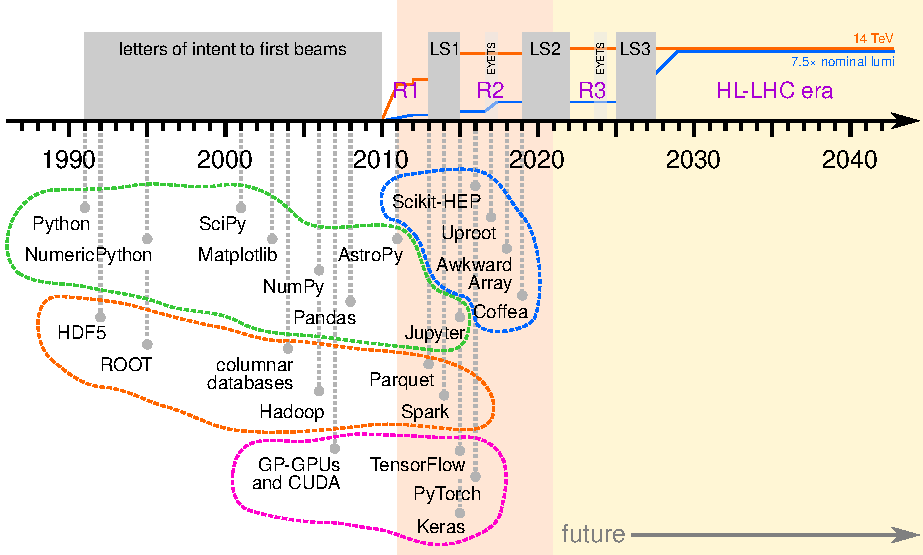
\includegraphics[width=0.9\linewidth]{hllhc-python-timeline-5.pdf}}
\end{center}
\end{frame}

\begin{frame}{Physicists have been moving to Python on their own}
\vspace{0.35 cm}

Primary language of GitHub repos created by users who forked CMSSW:

\vspace{-0.6 cm}
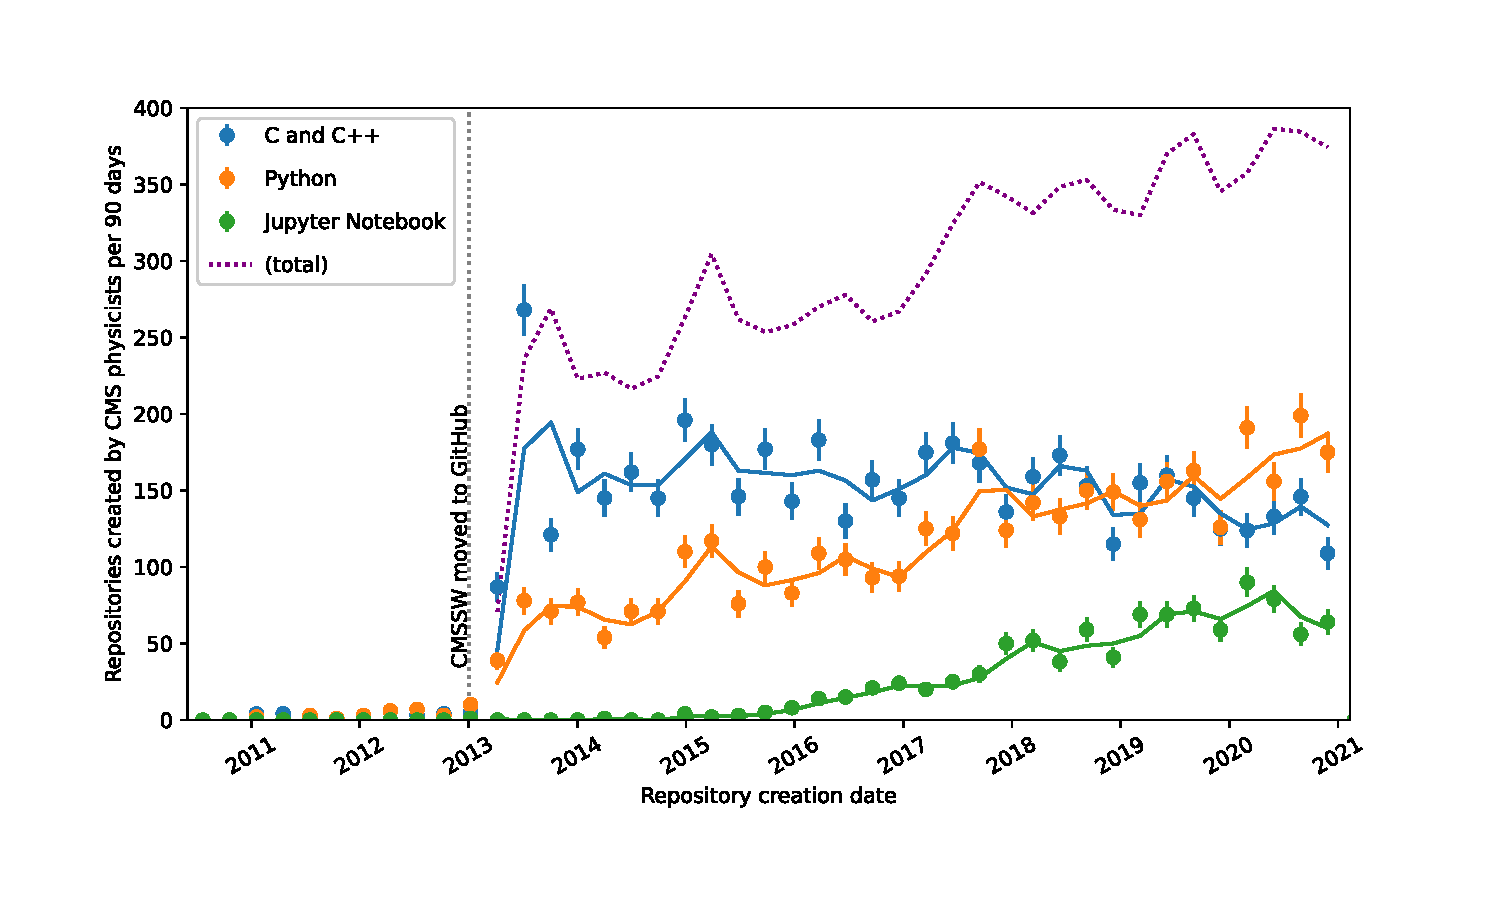
\includegraphics[width=\linewidth]{lhlhc-github-languages.pdf}
\end{frame}

\begin{frame}{Consistent with survey results (PyHEP 2020 participants)}
\vspace{0.2 cm}
\begin{columns}
\column{1.15\linewidth}
\only<1>{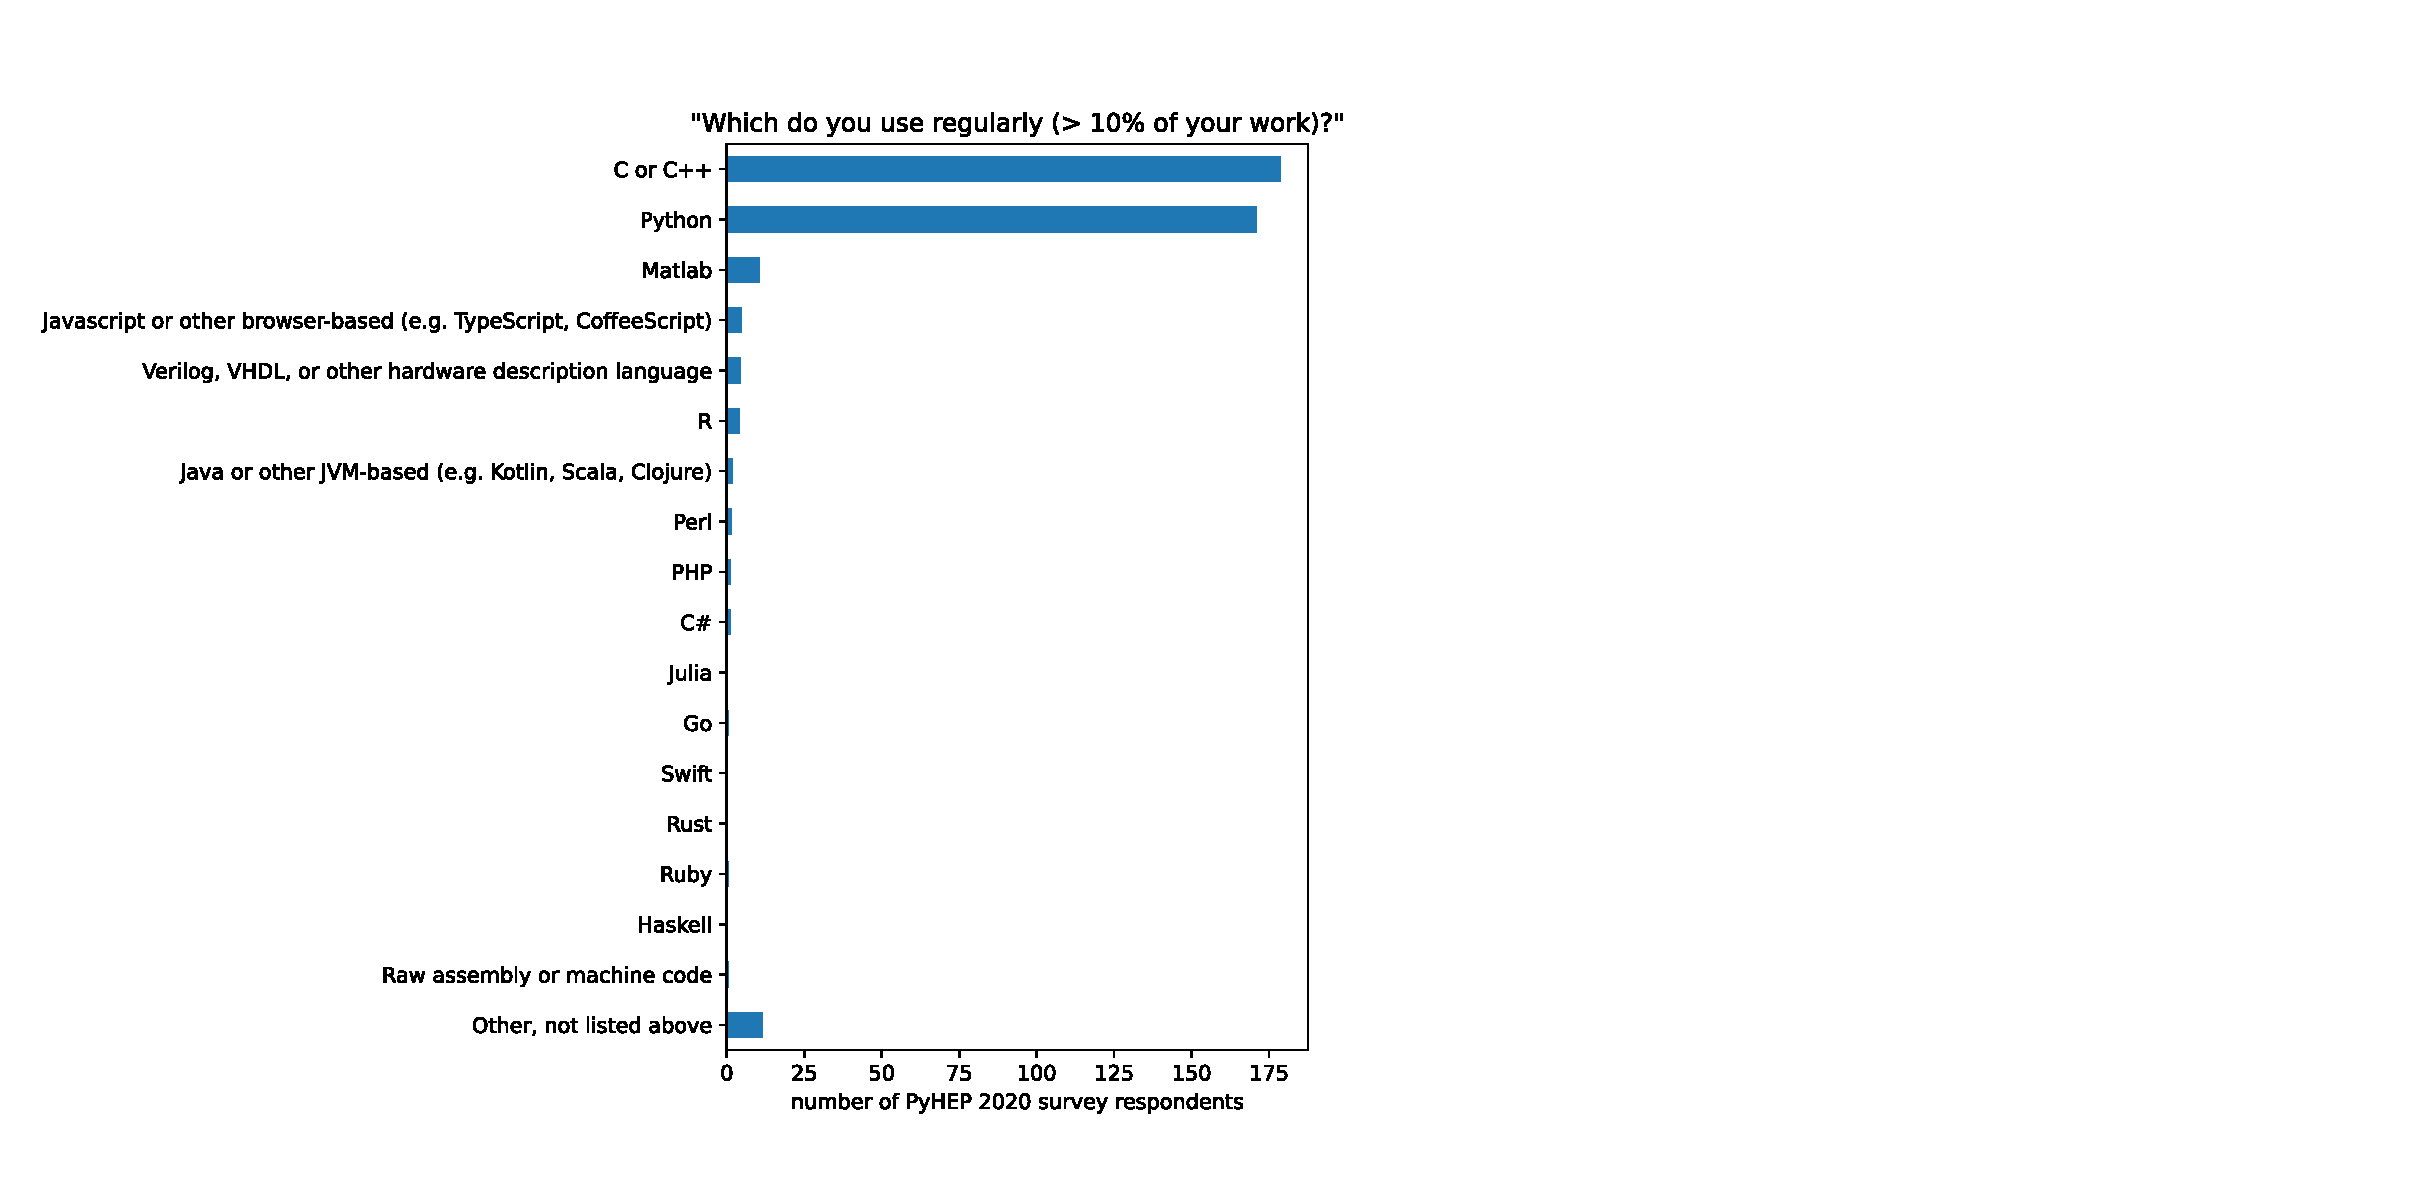
\includegraphics[width=\linewidth]{pyhep2020-survey-1.pdf}}\only<2>{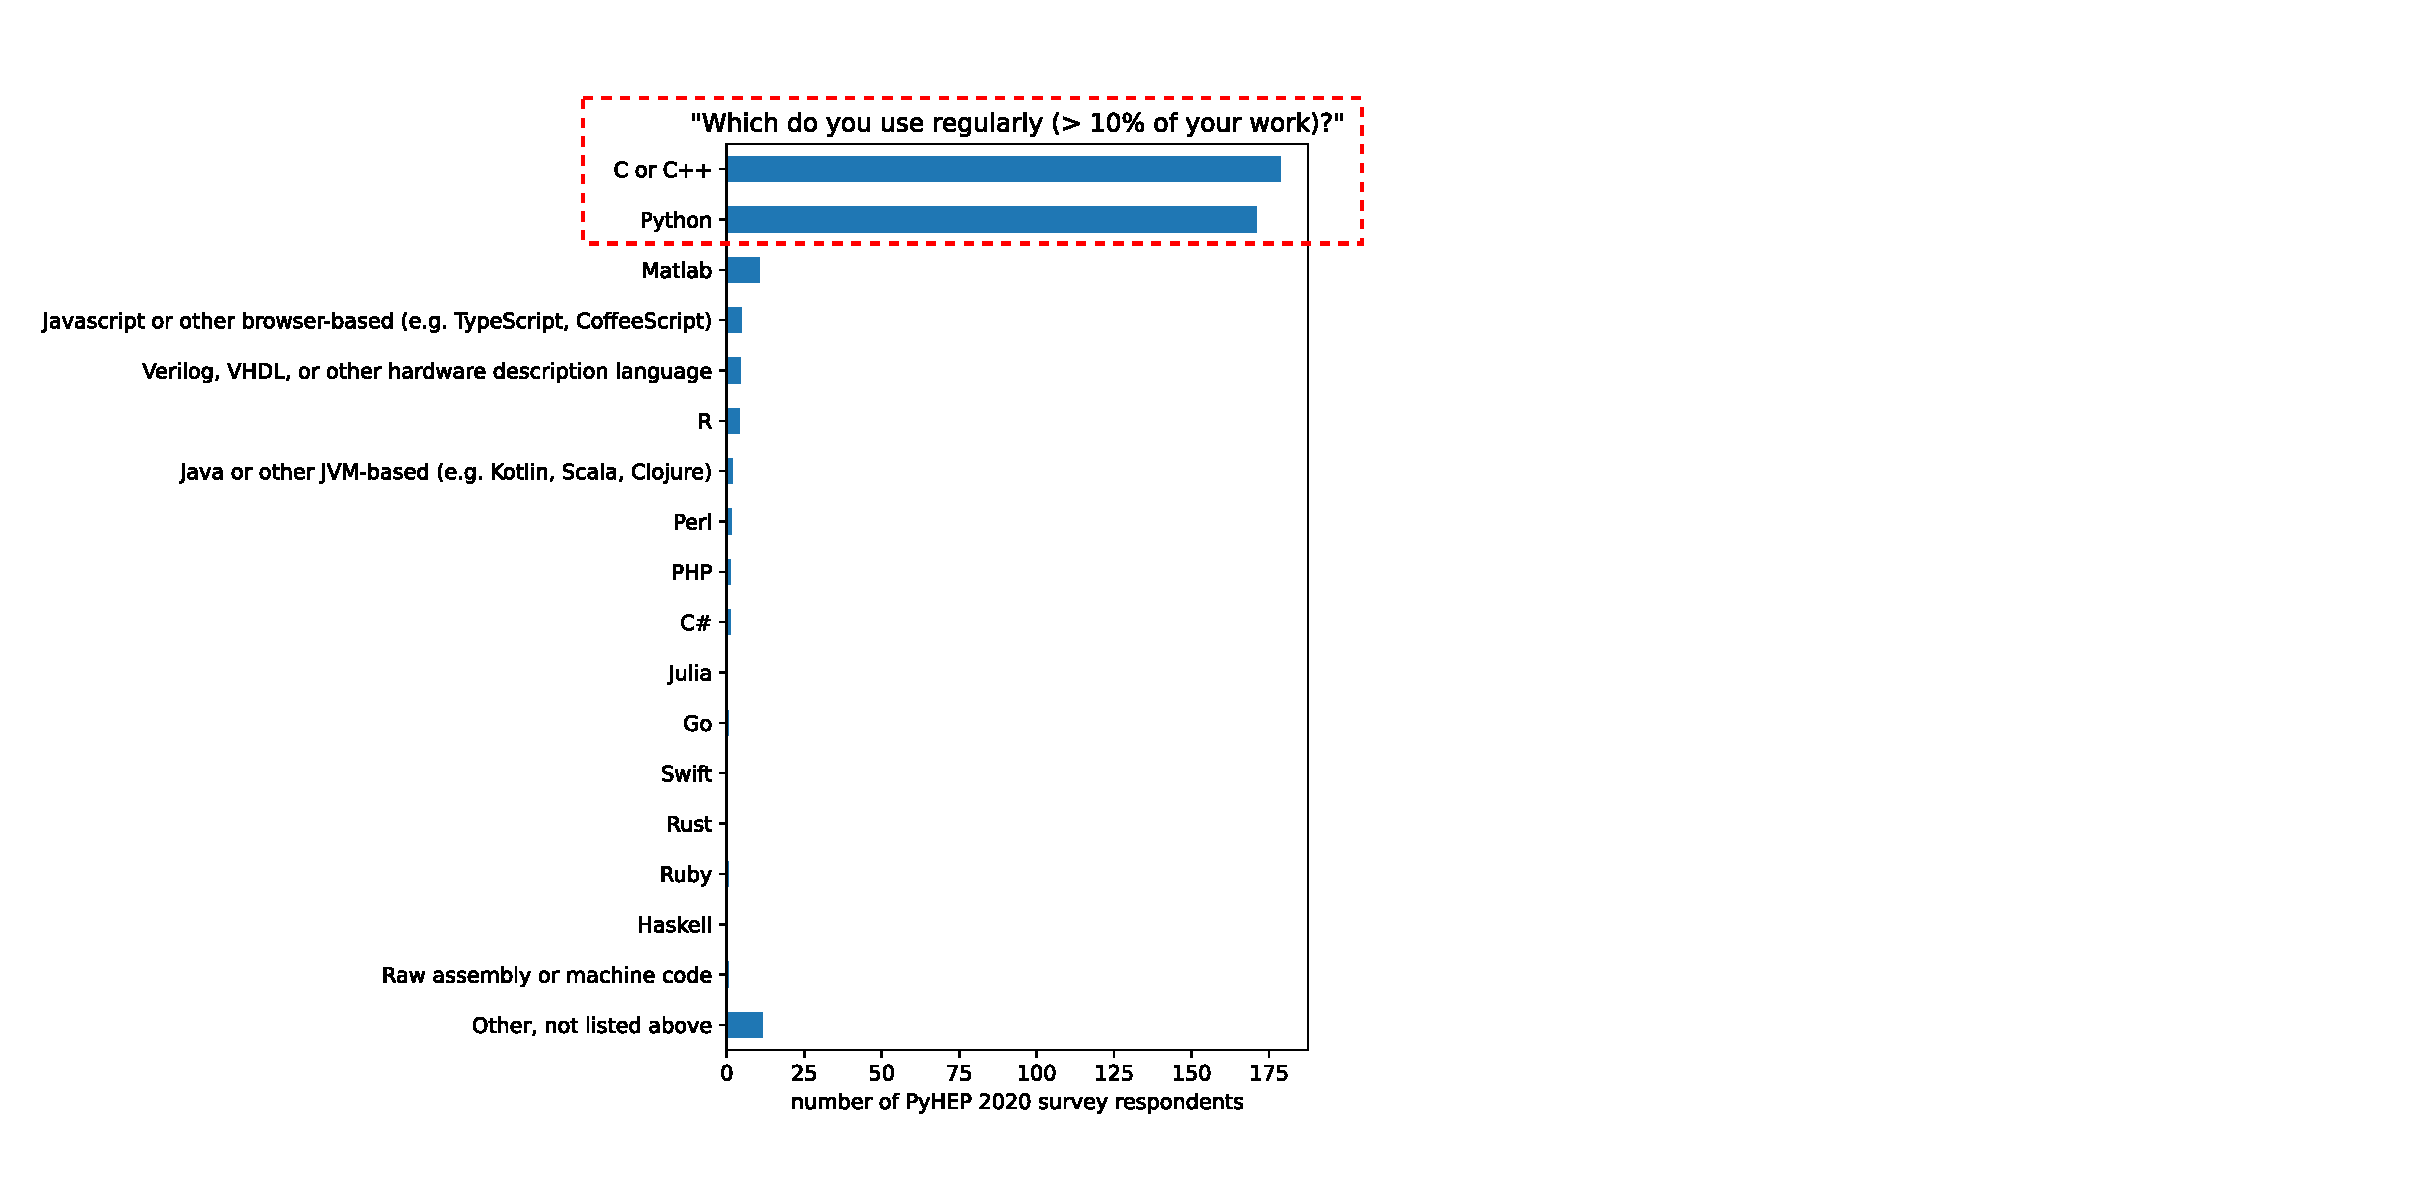
\includegraphics[width=\linewidth]{pyhep2020-survey-2.pdf}}\only<3>{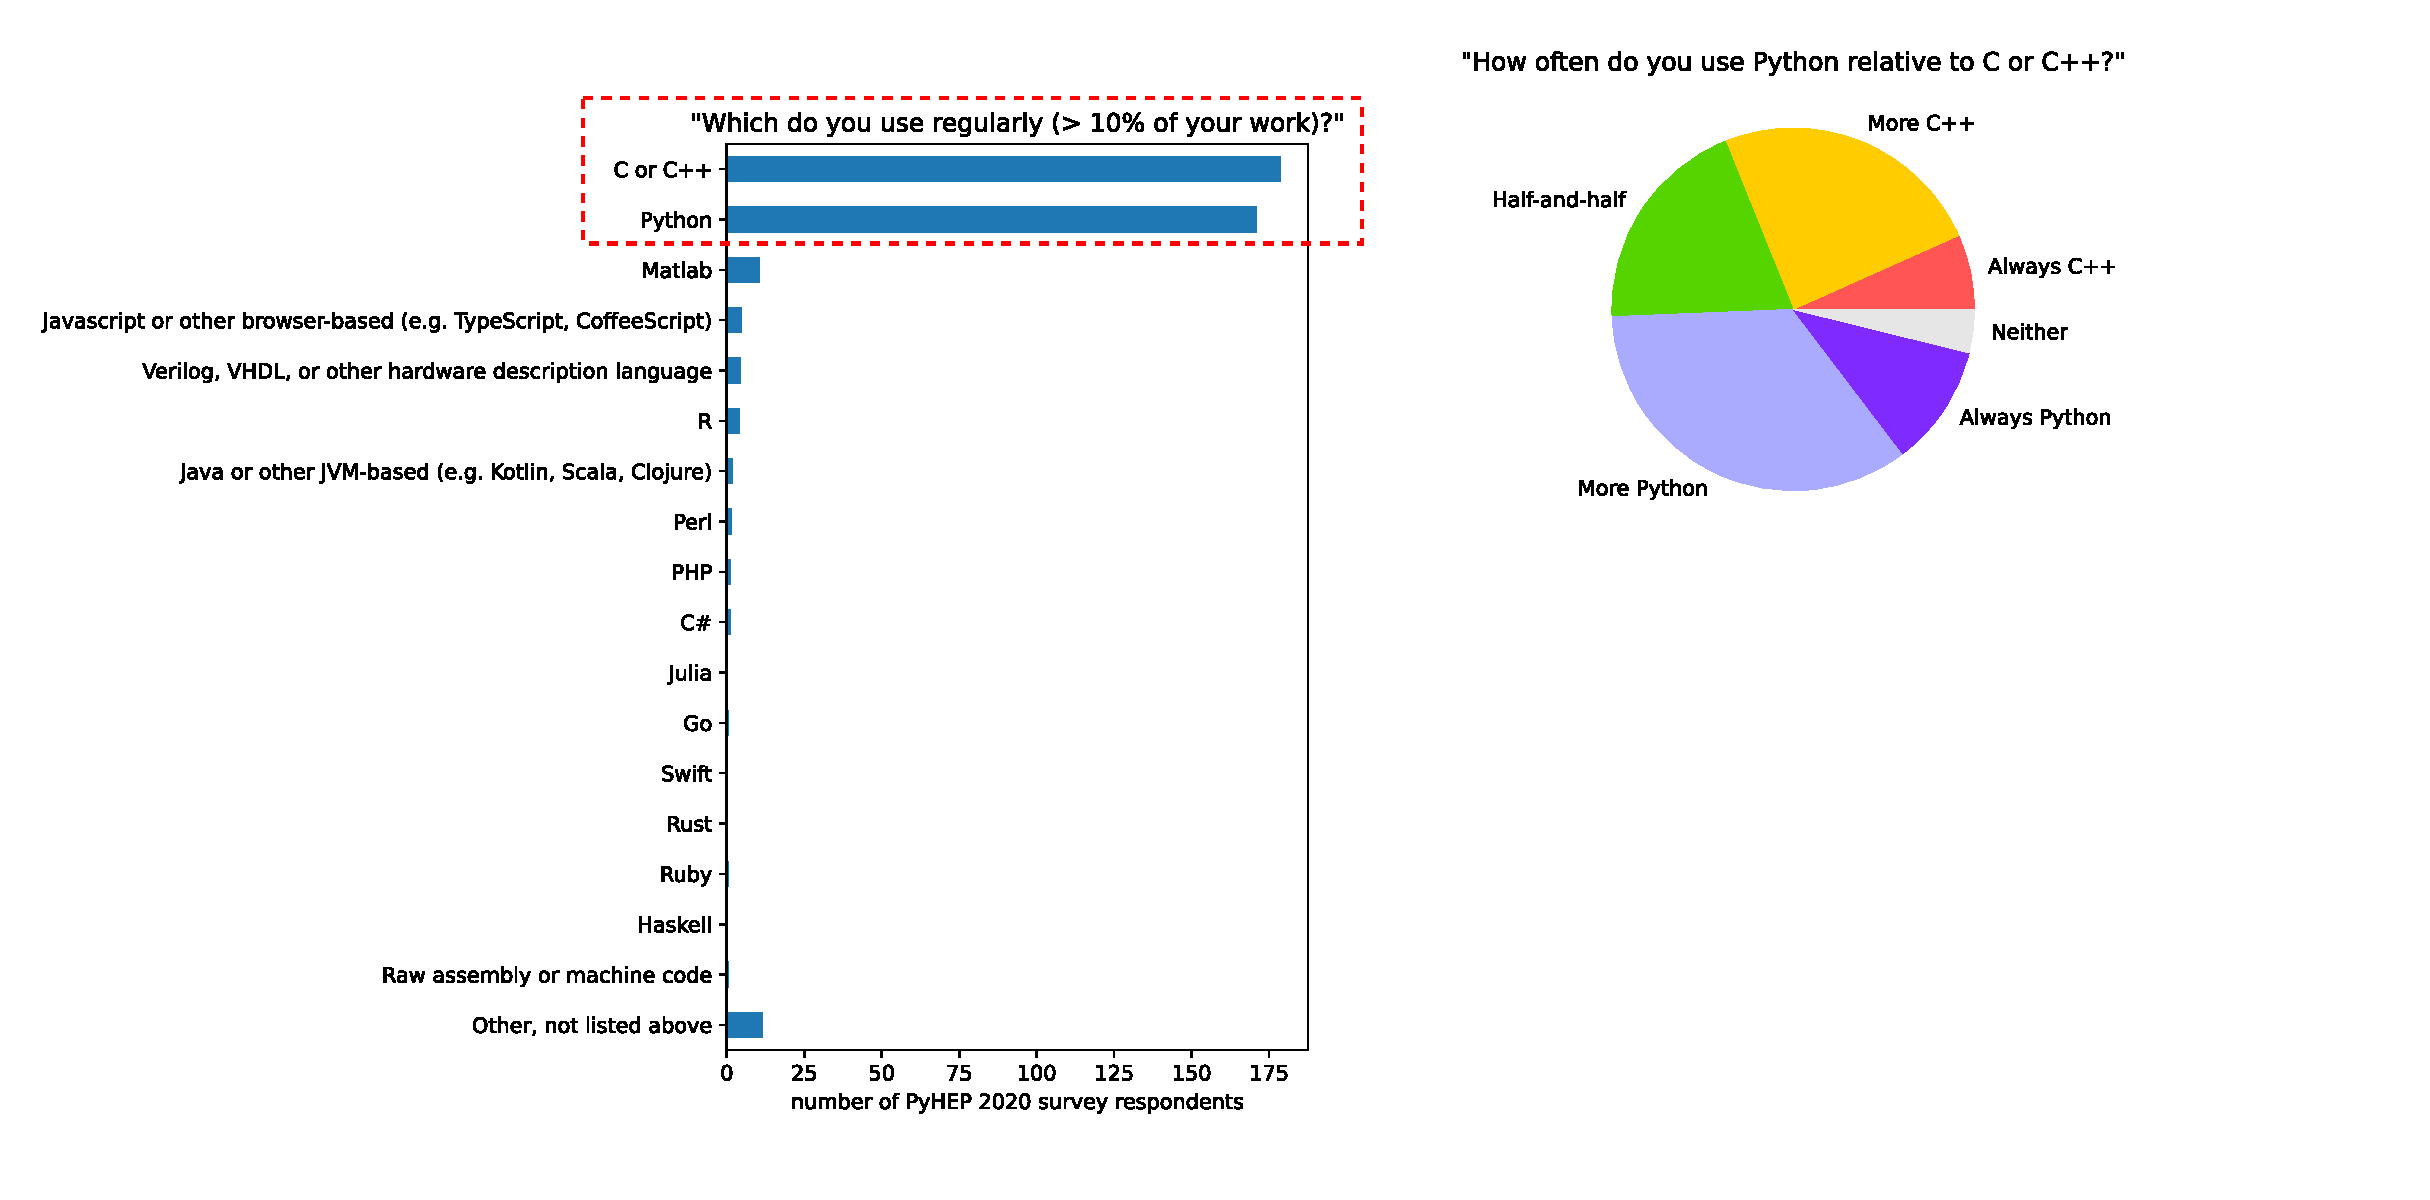
\includegraphics[width=\linewidth]{pyhep2020-survey-3.pdf}}\only<4>{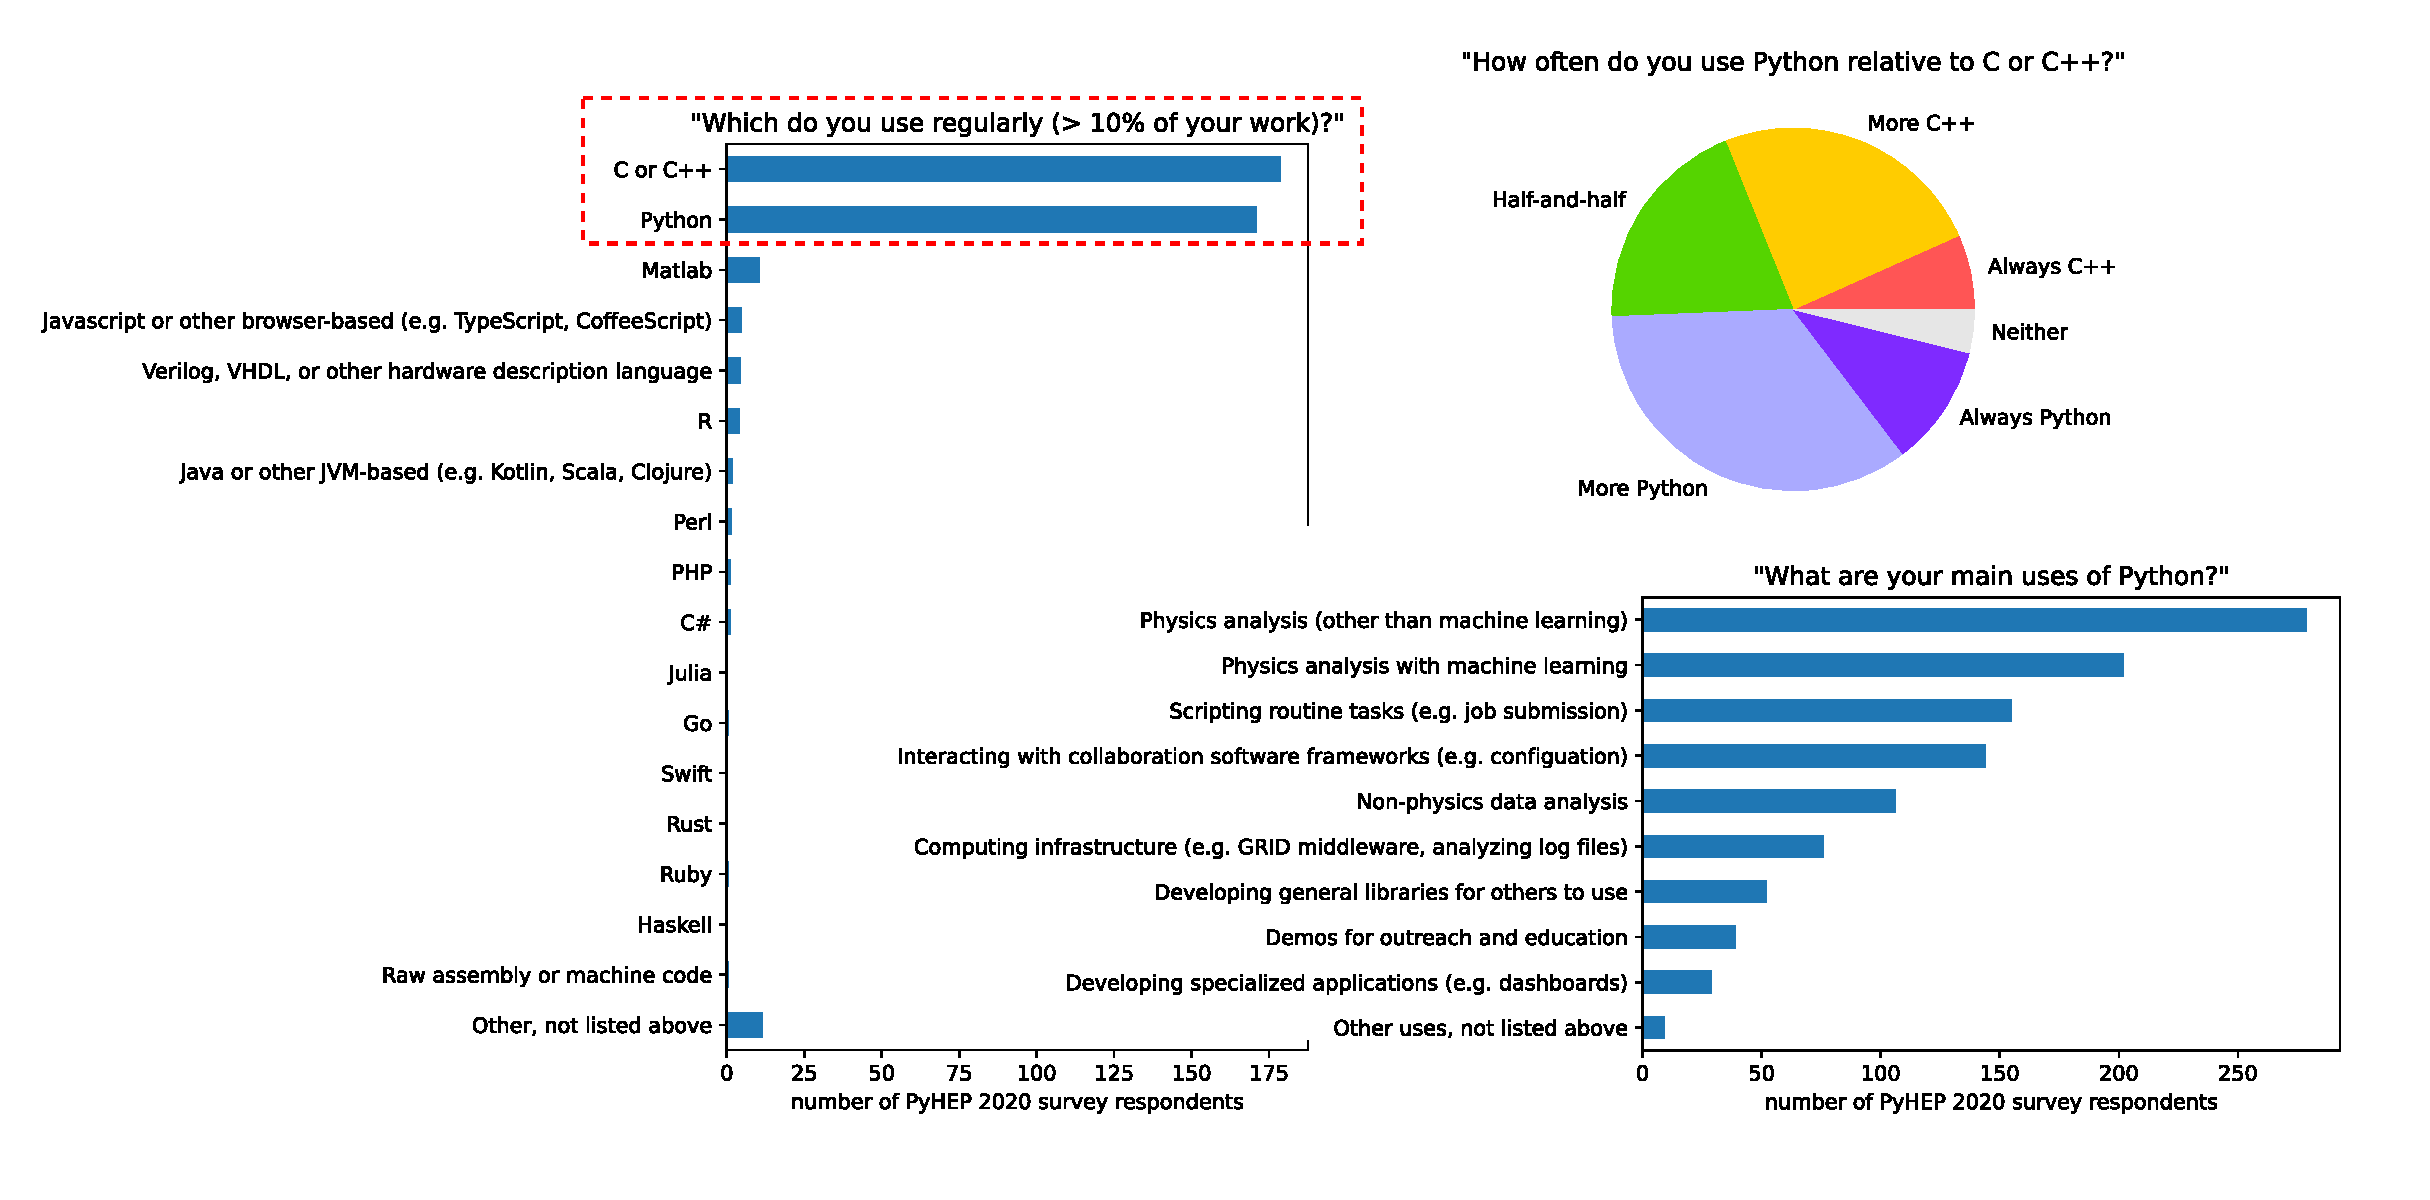
\includegraphics[width=\linewidth]{pyhep2020-survey-4.pdf}}\only<5>{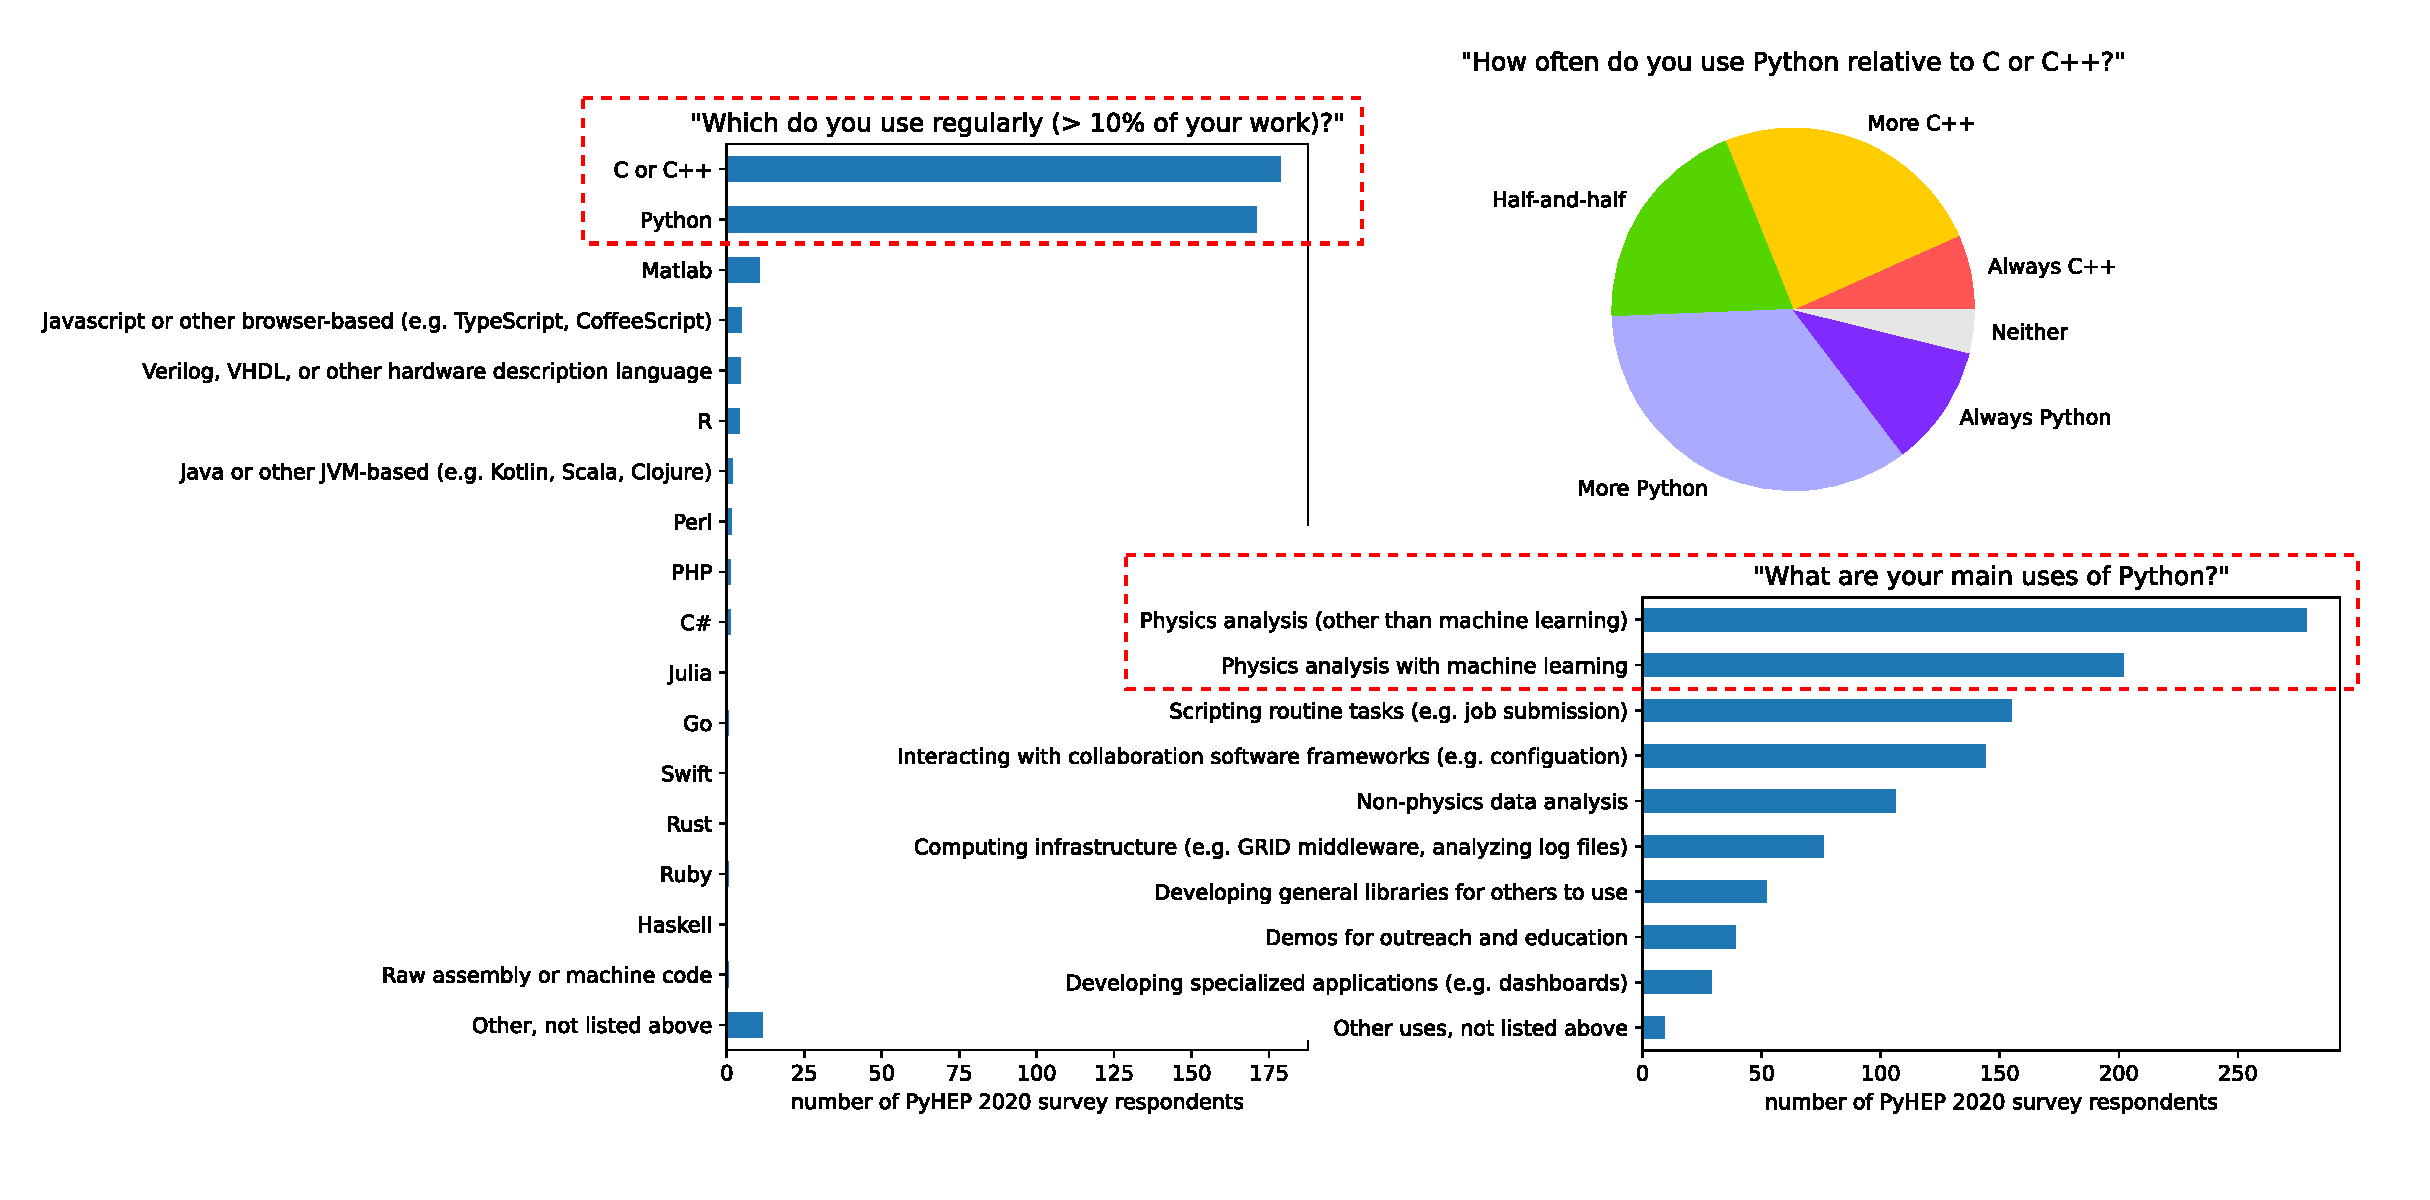
\includegraphics[width=\linewidth]{pyhep2020-survey-5.pdf}}
\end{columns}
\end{frame}

\begin{frame}{Pythonic analysis is mainstream, and the trend preceded Uproot}
\vspace{0.35 cm}

GitHub repos matching search strings: Pythonic analysis is as common as ``TFile''.

\vspace{-0.6 cm}
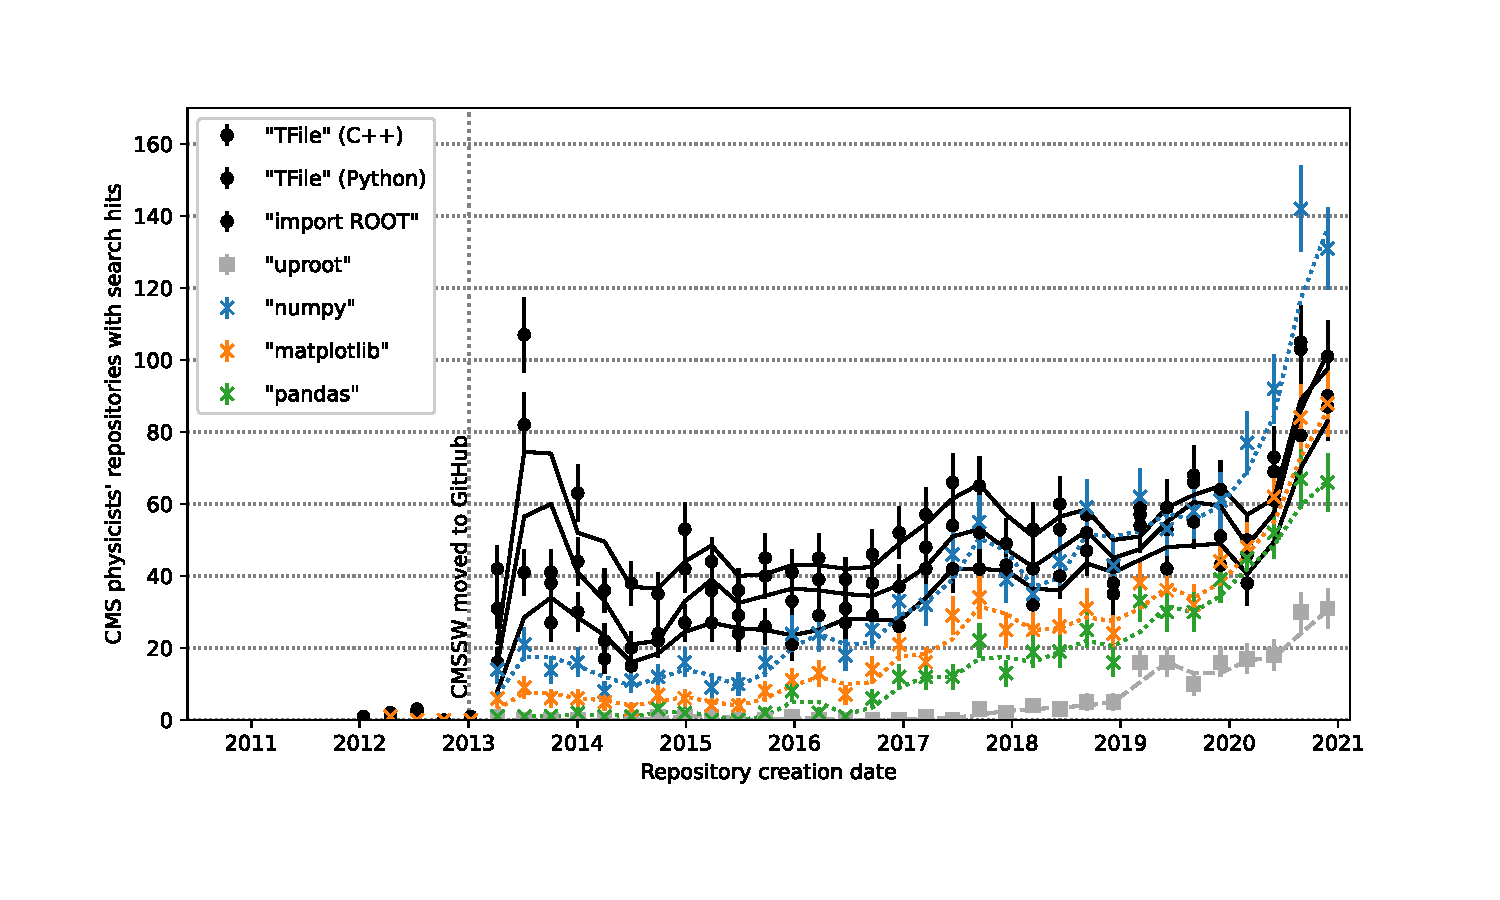
\includegraphics[width=\linewidth]{lhlhc-github-overlay-lin.pdf}
\end{frame}

\begin{frame}{This is also consistent with self-reported usage}
\vspace{-0.35 cm}
\begin{columns}
\column{1.1\linewidth}
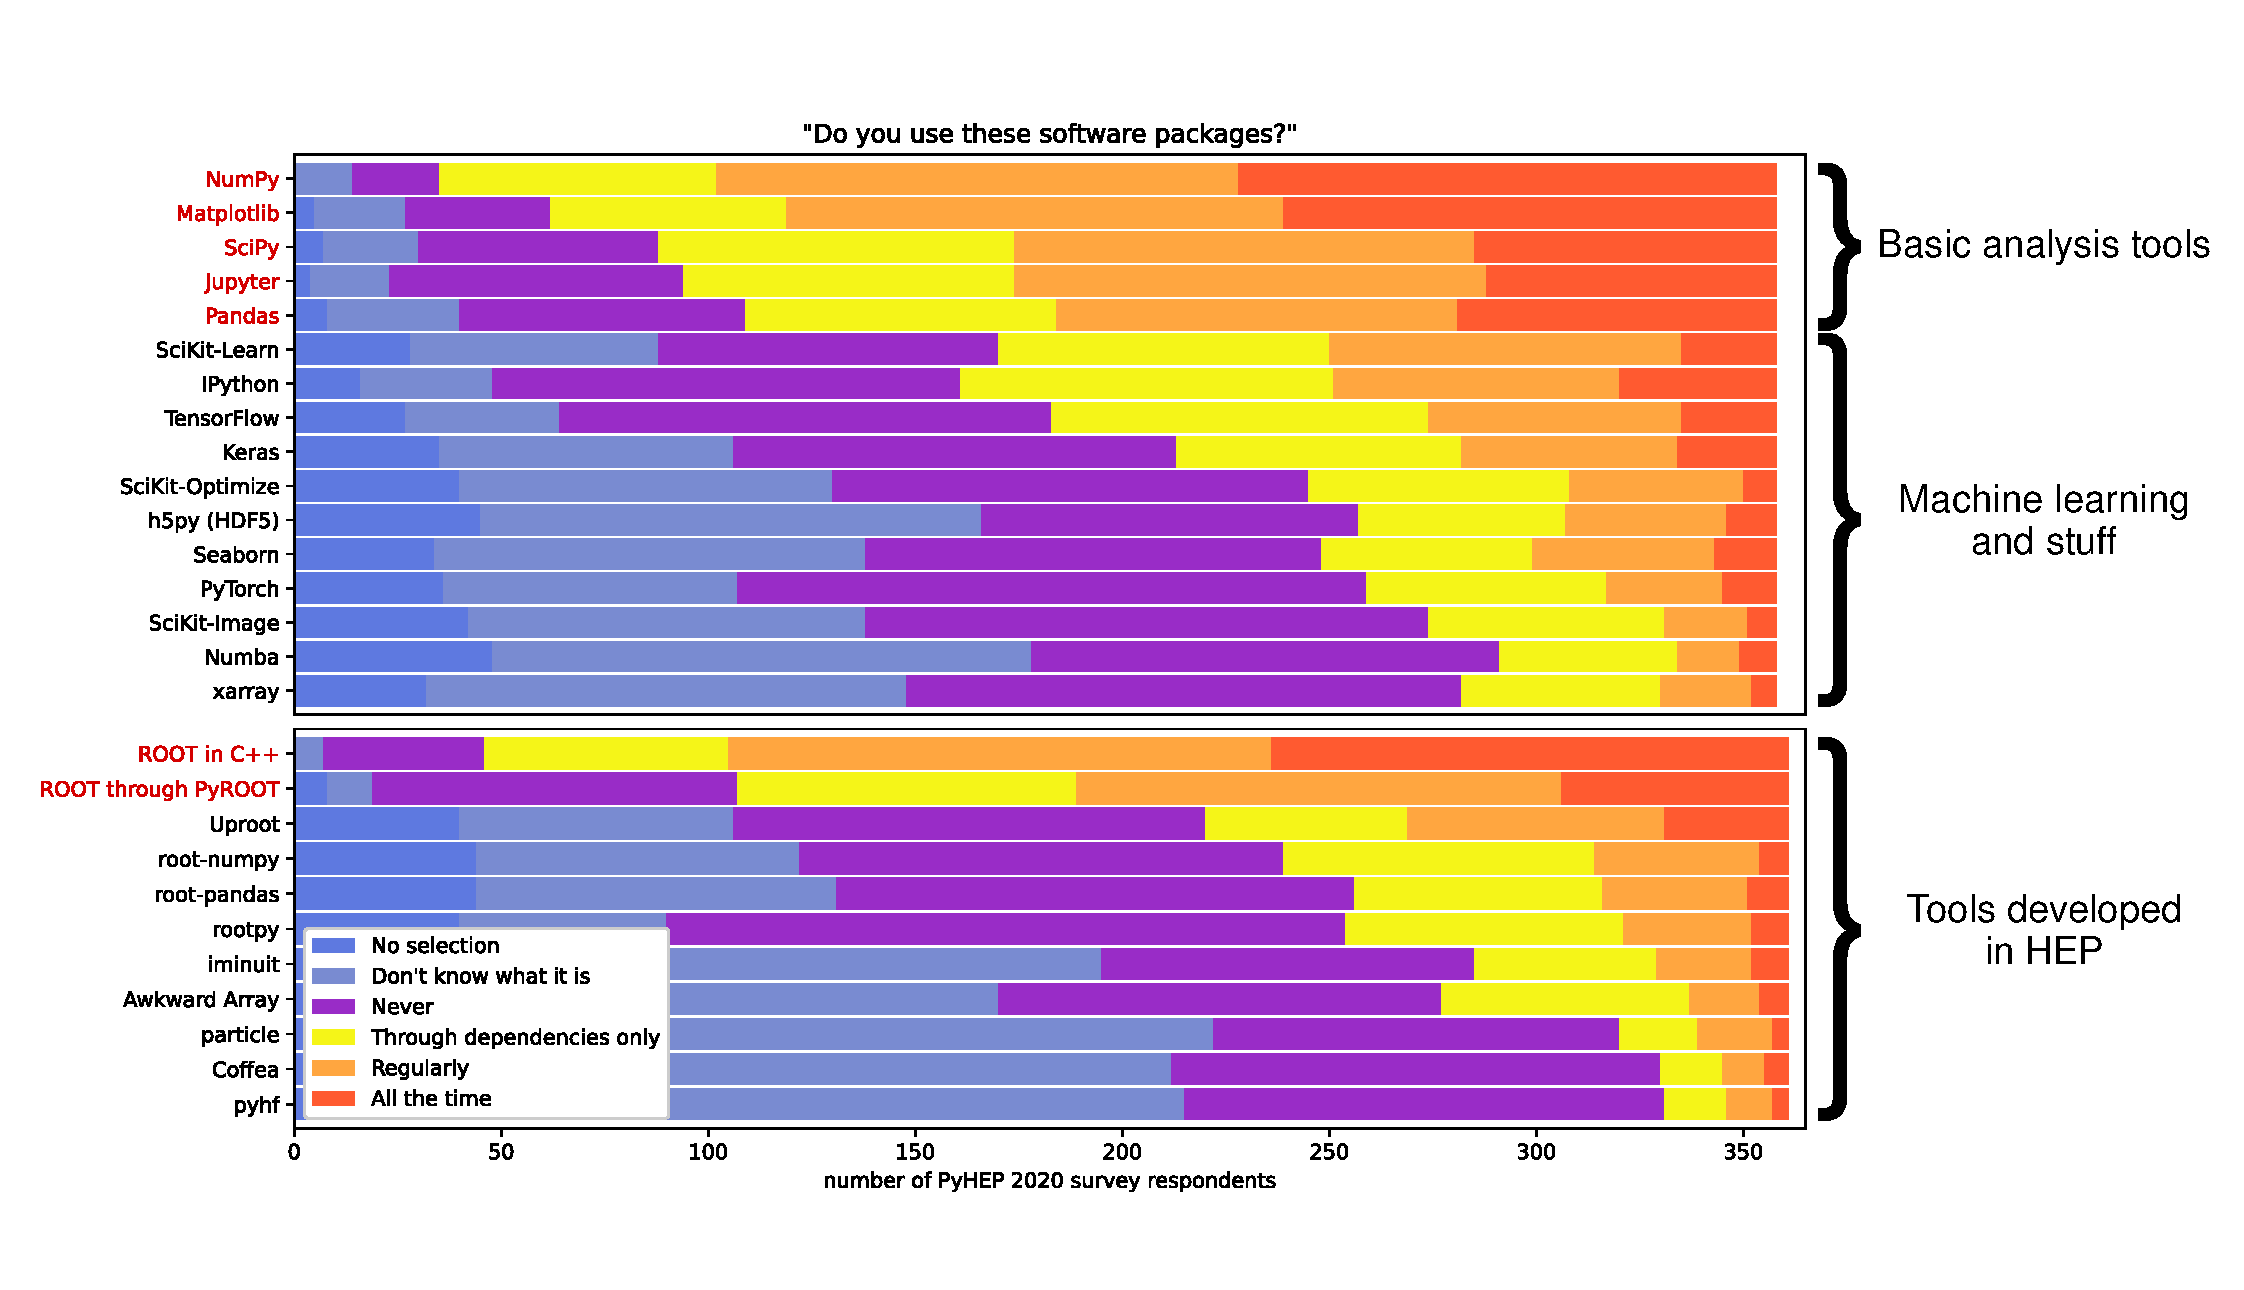
\includegraphics[width=\linewidth]{lhlhc-familiarity-with-packages.pdf}
\end{columns}
\end{frame}

\begin{frame}{}
\LARGE
\begin{center}
\textcolor{darkblue}{Part 2: Maturity of Python tools}
\end{center}
\end{frame}

\begin{frame}{Shared vision}
\vspace{0.4 cm}
\begin{center}
\begin{minipage}{0.83\linewidth}
\large
Most of the developers of Pythonic HEP software

\vspace{0.25 cm}
\begin{itemize}\setlength{\itemsep}{0.2 cm}
\item \textcolor{darkblue}{aim for small package granularity}, providing tools that address a well-defined class of problems at one level of abstraction,
\item \textcolor{darkblue}{aim for interoperability} with each other and the larger Pythonic ecosystem,
\item \textcolor{darkblue}{avoid overlapping functionality}, by communicating through HSF and IRIS-HEP channels,
\item \textcolor{darkblue}{focus on domain-specific problems} that won't be addressed by non-HEP software {\it or} \textcolor{darkblue}{connecting HEP-specific tools} to the larger ecosystem.
\end{itemize}
\end{minipage}
\end{center}
\end{frame}

%% \begin{frame}{Unshared vision}
%% \vspace{0.4 cm}
%% \begin{center}
%% \begin{minipage}{0.83\linewidth}
%% \large
%% Some people in this area are trying to replace ROOT.

%% \vspace{0.4 cm}
%% Others (myself included) are connect everything to everything, so that there are no artificial boundaries in data analysis.

%% \vspace{0.4 cm}
%% End-user analysis is a decentralized world. Small, interoperating tools have historically worked well in that environment.
%% \end{minipage}
%% \end{center}
%% \end{frame}

\begin{frame}{Scikit-HEP: clearinghouse for Pythonic HEP software}
\vspace{0.35 cm}
\begin{columns}
\column{0.8\linewidth}
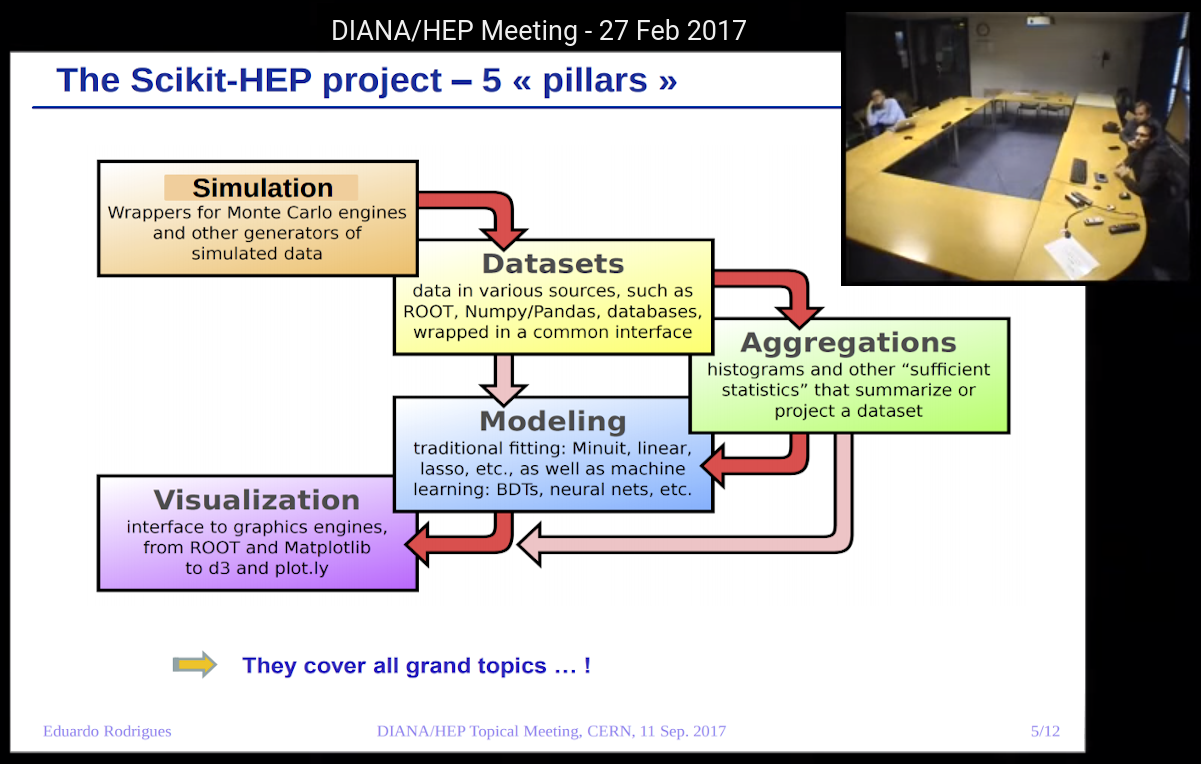
\includegraphics[width=\linewidth]{early-scikit-hep.png}
\column{0.27\linewidth}

Originally conceived as a core package with ``affiliates,'' now it's just the affiliates:

\vspace{0.2 cm}
a common brand for packages that work together and with the Python ecosystem.
\end{columns}
\end{frame}

\begin{frame}{Scikit-HEP's 5 pillars today:}
\vspace{0.3 cm}

\begin{description}
\item[Simulation:] other than \mintinline{python}{numpythia} and \mintinline{python}{pyhepmc}, this is mostly left to non-Python packages (which fill files that can be read with Python).

\item[Datasets:] \mintinline{python}{root-numpy}, \mintinline{python}{uproot}, \mintinline{python}{pylhe}, \mintinline{python}{awkward}, as well as \mintinline{python}{numpy} and \mintinline{python}{pandas}. Some use HDF5/\mintinline{python}{h5py} because of its recognition by ML tools.

\item[Aggregations:] \mintinline{python}{boost-histogram}/\mintinline{python}{hist}, \mintinline{python}{coffea}, \mintinline{python}{fast-carpenter}.

\item[Modeling:] by far, the most covered: \mintinline{python}{pyhf} (dozens of publications), \mintinline{python}{iminuit}, \mintinline{python}{zfit}, \mintinline{python}{hepstats}, \mintinline{python}{goofit}, \mintinline{python}{SModelS}, direct use of Pandas, ML\ldots

\item[Visualization:] most modeling tools output to \mintinline{python}{matplotlib}, \mintinline{python}{mplhep} is widely used as a dependency. \mintinline{python}{coffea}, \mintinline{python}{hist}, \mintinline{python}{histoprint}.

\end{description}

\vspace{0.25 cm}
Should also add \textcolor{darkblue}{Distributed computing:} some \mintinline{python}{pyspark}, but more \mintinline{python}{dask}, often through \mintinline{python}{coffea} (future \mintinline{python}{coffea-casa}/ServiceX).

\vspace{0.25 cm}
Should also add \textcolor{darkblue}{Acceleration:} \mintinline{python}{numba} and \mintinline{python}{ROOT.RDataFrame}.

\vspace{0.25 cm}
\textcolor{darkblue}{Other:} corrections in \mintinline{python}{coffea}, Lorentz vectors in \mintinline{python}{vector}, PDG in \mintinline{python}{particle}\ldots
\end{frame}





\end{document}
